%%%%%%%%%%%%%%%%%%%%%%%%%%%%%%%%%%%%%%%%%%%%%%%%%%%%%%%%%%%%%%%%%%%%%%
% How to use writeLaTeX: 
%
% You edit the source code here on the left, and the preview on the
% right shows you the result within a few seconds.
%
% Bookmark this page and share the URL with your co-authors. They can
% edit at the same time!
%
% You can upload figures, bibliographies, custom classes and
% styles using the files menu.
%
%%%%%%%%%%%%%%%%%%%%%%%%%%%%%%%%%%%%%%%%%%%%%%%%%%%%%%%%%%%%%%%%%%%%%%

\documentclass[12pt]{article}

\usepackage{sbc-template}

\usepackage{graphicx,url}

\usepackage[brazil]{babel}   
\usepackage[utf8]{inputenc}  
     
\sloppy

\title{Gestão Pessoal de Credenciais de Acesso a Serviços Digitais}

\author{Felipe Juris Jacques\inst{1}, Eduardo Dalcin\inst{1} }

\address{
  Especialização em Gestão de Tecnologia da Informação
  \\
  Instituto Federal de Educação, Ciência e Tecnologia Farroupilha Campus Panambi
  \\
  (IFFAR) -- Caixa Postal 98787 -- 740 -- Panambi -- RS -- Brazil
}

\begin{document} 

\maketitle

\begin{abstract}
  This meta-paper describes the style to be used in articles and short papers
  for SBC conferences. For papers in English, you should add just an abstract
  while for the papers in Portuguese, we also ask for an abstract in
  Portuguese (``resumo''). In both cases, abstracts should not have more than
  10 lines and must be in the first page of the paper.
\end{abstract}
     
\begin{resumo} 
  Este meta-artigo descreve o estilo a ser usado na confecção de artigos e
  resumos de artigos para publicação nos anais das conferências organizadas
  pela SBC. É solicitada a escrita de resumo e abstract apenas para os artigos
  escritos em português. Artigos em inglês deverão apresentar apenas abstract.
  Nos dois casos, o autor deve tomar cuidado para que o resumo (e o abstract)
  não ultrapassem 10 linhas cada, sendo que ambos devem estar na primeira
  página do artigo.
\end{resumo}


\section{Introdução}

All full papers and posters (short papers) submitted to some SBC conference,
including any supporting documents, should be written in English or in
Portuguese. The format paper should be A4 with single column, 3.5 cm for upper
margin, 2.5 cm for bottom margin and 3.0 cm for lateral margins, without
headers or footers. The main font must be Times, 12 point nominal size, with 6
points of space before each paragraph. Page numbers must be suppressed.

Full papers must respect the page limits defined by the conference.
Conferences that publish just abstracts ask for \textbf{one}-page texts.

\section{Credenciais de Acesso a Serviços Digitais} \label{sec:firstpage}

Qualquer serviço digital que exija autenticidade para identificar usuários
utiliza credenciais de acesso.
Embora cada serviço tenha credenciais únicas, eles compartilham padrões
comuns que os usuários conhecem.
Além disso, os serviços digitais têm contratos que os usuários devem aceitar, mas a
tecnologia por trás da segurança não é transparente para os usuários.
No entanto, é responsabilidade do usuário operar corretamente e respeitar
práticas de segurança comuns.

\subsection{A Segurança de Um Serviço Digital}

As credenciais de acesso devem ser protegidas para evitar que terceiros
mal-intencionados as usem para obter vantagens indevidas.
Ao se cadastrar em um serviço digital, é comum fornecer informações
pessoais de identificação.
É importante fornecer apenas informações necessárias e verdadeiras,
considerando quem terá acesso a elas. Deixar credenciais vulneráveis pode
expor o usuário a riscos ilimitados, como roubo de informações, extorsão,
invasão e mais.
É fundamental proteger as credenciais e informar apenas o mínimo necessário
para minimizar a exposição pessoal.

\section{Processo de Autenticação}

Quando um usuário acessa um serviço digital, ele faz isso por meio do
processo de autenticação (login), fornecendo duas informações: uma
identificação única (telefone, nome ou e-mail) e uma senha secreta.
É fundamental que a senha seja aleatória e não contenha informações
que possam ser facilmente memorizadas e principalmente, não deve conter
informações pessoais, pois isso pode ser descoberto por pessoas
mal-intencionadas.
Além disso, informações pessoais podem ser obtidas de várias maneiras,
como em perfis públicos do usuário.

\subsection{Multi Fator de Autenticação}

A autenticação multifator (MFA) é uma medida de segurança adicional que
exige dois ou mais fatores de verificação para acessar uma conta ou
recurso online.
Isso aumenta a dificuldade de acesso não autorizado, pois mesmo com a
senha, o atacante precisaria de um segundo fator, como um código
enviado ao smartphone, uma impressão digital ou outro tipo de
verificação adicional.
A MFA se tornou uma prática padrão em serviços digitais, como bancos,
redes sociais e sistemas corporativos, fornecendo uma camada adicional
de segurança contra roubo de identidade e fraude cibernética.

\subsection{Duplo Fator de Autenticação}

O duplo fator de autenticação (2FA) é uma medida de segurança adicional
que exige um segundo fator além da senha, como um código enviado ao
celular ou um token de hardware.
Isso torna mais difícil para os atacantes acessarem contas online, mesmo
que eles obtenham a senha.
Muitos serviços online oferecem 2FA como opção para aumentar a segurança
dos usuários.
Ativar o 2FA é uma etapa importante para proteger informações pessoais e
é recomendável habilitá-lo sempre.
Além disso, é possível usar múltiplos hardwares e é indispensável
realizar backup em nuvem ou arquivo digital. No entanto, alguns serviços
não oferecem 2FA ou exigem aplicativos proprietários, então é importante
estar atento aos recursos de recuperação de acesso.

\section{Phishing}

Phishing é um tipo de ataque cibernético onde criminosos tentam obter
vantagem ou obter informações confidenciais, como senhas, informações
pessoais e até detalhes de cartões de crédito, por meio de comunicações
fraudulentas.
Este termo deriva da palavra "fishing", que significa pescar em inglês,
aludindo à ideia de lançar iscas para capturar vítimas desavisadas.

Os ataques de phishing podem ocorrer através de e-mails, mensagens de
texto e chamadas telefônicas fraudulentas, serviços online falsos que
se assemelham muito com os verdadeiros, aplicativos malignos em lojas
de aplicativos, postagens e propagandas enganosas em redes sociais e
anúncios fraudulentos de internet, onde os golpistas se passam por
entidades legítimas para persuadir as pessoas a fornecerem suas informações
pessoais ou tirar vantagens para realizar ataques ao dispositivo.

A conscientização sobre esses golpes é crucial, pois o conhecimento é a
primeira linha de defesa contra os ataques cibernéticos.
É importante estar atento a mensagens suspeitas que solicitam dados
confidenciais ou contêm links e anexos desconhecidos. Para se proteger,
verifique a autenticidade das mensagens, não clique em links ou baixe
anexos de fontes desconhecidas e use soluções de segurança confiáveis.
Se receber um código de autenticação sem solicitar, não o informe a
ninguém e altere sua senha, pois pode ser uma tentativa de invasão.

\section{Multiplas Credencais de Acesso}

É comum que os usuários precisem gerenciar muitas credenciais de acesso
para diversos serviços online.
Nessa situação, não é recomendado repetir senhas para evitar que um invasor
descubra uma senha e acesse outros serviços.
É importante ter uma boa gestão de senhas e credenciais, incluindo a
possibilidade de recuperar senhas esquecidas.

\subsection{Lugares para Guardar Anotações de Credênciais}

É improvável que uma pessoa possa memorizar todas as credenciais de acesso,
então é necessário anotar as informações em algum lugar.
É importante anotar não só o login e senha, mas também outros detalhes,
como códigos de recuperação e descrições.

Ao usar um meio digital para anotações, é desejável usar software ou
aplicativos de confiança para proteger as informações. Além disso, é útil
evitar letras e caracteres semelhantes para evitar confusões.

\subsubsection{Anotações em Meio Físico}

É comum optar por anotar as informações das credenciais de acesso em um
caderno, já que requer menos desafios de informatização.
Deve se ter atenção a senhaa, já que representar caracteres, letras
maiúsculas ou minúsculas pode ser mais difícil do que digitalmente e
causar confusões nos usuários mais despreparados.

Optar por anotar informações de credenciais de forma digital em arquivos
no computador pessoal, smartfone ou pendrive envolve complexidades pois
para fornecer algum tipo de segurança, requer criptografia e backups
atualizados para proteger arquivos e evitar que possam ser acessados por
usuários indesejados.

\subsubsection{Anotações em Serviços de Terceiros}

Criptografar arquivos manualmente é desafiador e arriscado, porém,
existem softwares de terceiros que podem auxiliar nessa tarefa de gerir
arquivos com informações possais.
Uma maneira mais simples é fazer uso de serviços de terceiros que
oferecem softwares e aplicativos para gerenciar logins e senhas de
credenciais.
Mas antes de tudo, o usuário deve estar atento aos termos de uso de
qualquer serviço de software.

Existem diversos aplicativos, softwares ou até projetos para gerir
credenciais de acesso, um deles é o projeto de código aberto multi
plataforma KeeWeb que pode ser replicado, instalado em seu computador ou
servidor pessoal ou mesmo usar gratuitamente na internet.
KeeWeb não é um serviço, portanto não coleta suas informações, cabe ao
usuário optar em salvar em uma nuvem de uso pessoal ou no próprio
dispositivo pessoal, já que o mesmo gera arquivos que estão sempre
criptografados, podendo ser uma alternativa segura aos usuários que
pretendem carregar o arquivo criptografado consigo mesmo.

Normalmente as empresas privadas que oferecem softwares de assinatura
para anti vírus, também podem oferecer serviços para gestão de
credenciais de acesso, como por exemplo a Kaspersky que oferece o
Kaspersky Password Manager.


O usuário deve evitar anotar senhas em no celular em aplicativos de
bloco de notas, como contato de ligações telefônicas, aplicativos de
mensagens em geral, inclusive WhatsApp, pois todos esses recursos não são
criptografados e normalmente são protegidos para esses fins e podem ser
explorados por quem tiver acesso ao dispositivo.

\subsection{Anotações em Nuvem}

É muito comum os usuários fazerem uso dos serviços de terceiros,
oferecidos pelo Google, Microsoft, Opera e até outras empresas que
possuem algum sistema operacional para computadores ou navegadores de
internet.
Muitas vezes os usuários já estão fazendo o uso desses serviços para
anotarem seus logins e senhas sem se darem por conta, já que aquele botão
que aparece automaticamente para salvar o login e a senha é muito prático
de se utilizar até mesmo de forma desatenta, o que requer atenção
redobrada ao utilizar um dispositivo que não seja de uso pessoal.

Normalmente não há custo sobre esses serviços que estão embutidos em
sistema operacionais ou navegadores de internet.
Somente se o usuário estiver autenticado com uma credencial vinculada ao
mesmo, haverá a opção de ter seus logins e senhas salvos em nuvem e
sincronizados em seus dispositivos levando a praticidade de realizar a
autenticação sem necessariamente fazer conhecimento do login ou da senha.

O Google permite salvar logins e senhas em dispositivos com sistema
operacional Android ou no navegador de internet Chrome, o usuário poderá
visualizar e editar os logins e senhas online nas configurações da
própria conta.
Já a Microsoft disponibiliza salvar as mesmas informações diretamente no
navegador de internet Edge, o usuário poderá visualizar e editar os
logins e senhas através do aplicativo Microsoft Autenticador que também
é um aplicativo utilizando para 2FA, sendo essa uma opção cômoda aos
usuários que pretendem gerenciar as duas informações em um mesmo lugar.
Ambos os casos citados não permitem anotar mais detalhes além de login e
senha das respectivas credenciais de acesso sendo um fator limitante,
principalmente ao anotar descrições, pins e histórico de senhas,
inclusive essas informações não estão protegidas nos navegadores de
internet e estão protegidas por uma senha simples e curta nos sistemas
operacionais, portanto, o 2FA se torna crucial para as credenciais de
acesso salvas nesses serviços.

\section{Trabalhos Relacionados}

Araujo et al. (2015), em seu artigo sobre a influência da Lei de Zipf na
escolha de senhas, analisa a criação de senhas seguras considerando a
teoria da informação e a lei de Zipf.
A lei de Zipf, que descreve a relação entre a frequência de ocorrência de
palavras e sua posição em uma lista ordenada, reduz a entropia das senhas
quando linguagens naturais são utilizadas, criando padrões que podem ser
explorados por atacantes.
A pesquisa conclui que a estratégia mais eficaz para criar senhas robustas
é a utilização de acrônimos, que aumenta a entropia por caractere em
aproximadamente 80%.
Outras estratégias, como o uso de palavras isoladas, passphrases e o
método Diceware, mostraram-se menos eficazes.
O estudo destaca a importância de escolher senhas que maximizem o espaço
de busca para ataques de força bruta, especialmente em sistemas com
restrições de comprimento.

Araujo et al. (2015), relata limitações de segurança em algum serviços
digitais na conclusão de seu artigo:
\begin{quote}
  Conforme observado em, 'Muitas vezes os sistemas restringem o comprimento da chave, por exemplo, a
  Microsoft restringe a 16 caracteres, muitas lojas de comércio eletrônico também restringem drasticamente o
  número de caracteres de uma senha. Lojas virtuais como Submarino e Americanas.com utilizam o máximo de 8
  caracteres, enquanto Netshoes utiliza 15 e, ainda, Mercado Livre, 20. Mais grave ainda são os bancos que,
  além de restringir o tamanho de sua senha, restringem também o alfabeto, aceitando apenas dígitos de 0 a 9.
  Essa prática de restringir o tamanho e tipo de caracteres nas senhas pode levar à criação de senhas mais
  fracas e, portanto, mais vulneráveis a ataques. \cite{araujo:2015}
\end{quote}

\section{Figures and Captions}\label{sec:figs}


Figure and table captions should be centered if less than one line
(Figure~\ref{fig:exampleFig1}), otherwise justified and indented by 0.8cm on
both margins, as shown in Figure~\ref{fig:exampleFig2}. The caption font must
be Helvetica, 10 point, boldface, with 6 points of space before and after each
caption.

\begin{figure}[ht]
\centering
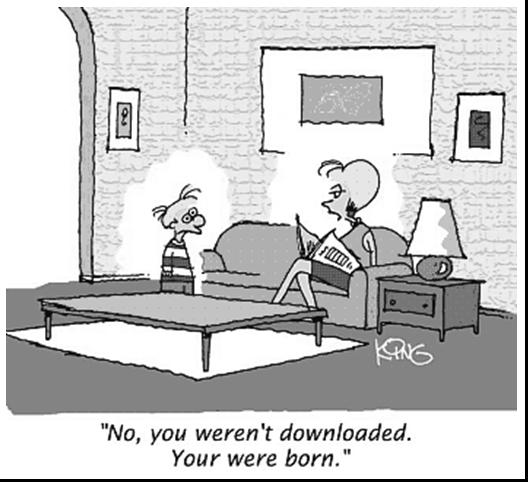
\includegraphics[width=.5\textwidth]{fig1.jpg}
\caption{A typical figure}
\label{fig:exampleFig1}
\end{figure}

\begin{figure}[ht]
\centering
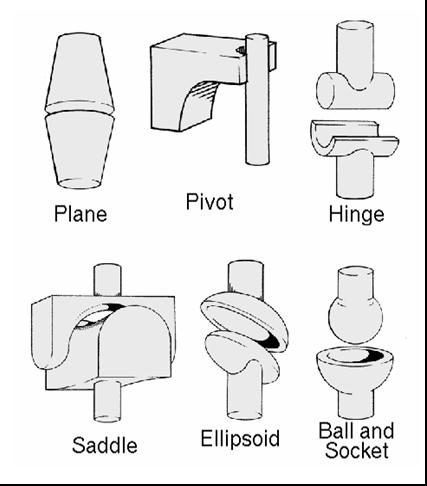
\includegraphics[width=.3\textwidth]{fig2.jpg}
\caption{This figure is an example of a figure caption taking more than one
  line and justified considering margins mentioned in Section~\ref{sec:figs}.}
\label{fig:exampleFig2}
\end{figure}

In tables, try to avoid the use of colored or shaded backgrounds, and avoid
thick, doubled, or unnecessary framing lines. When reporting empirical data,
do not use more decimal digits than warranted by their precision and
reproducibility. Table caption must be placed before the table (see Table 1)
and the font used must also be Helvetica, 10 point, boldface, with 6 points of
space before and after each caption.

\begin{table}[ht]
\centering
\caption{Variables to be considered on the evaluation of interaction
  techniques}
\label{tab:exTable1}
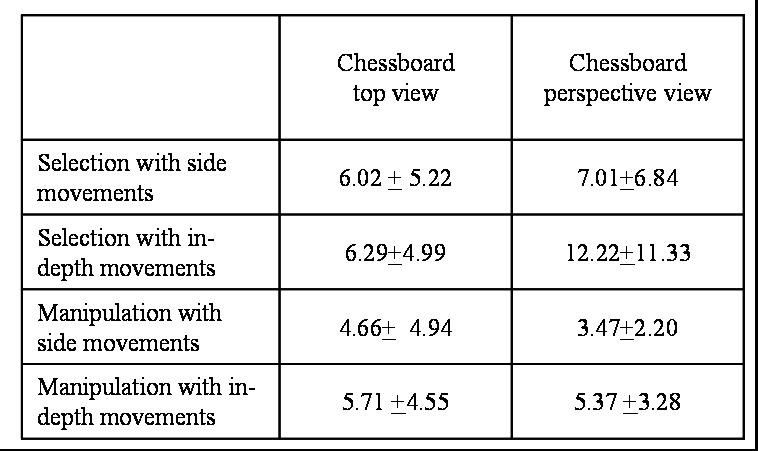
\includegraphics[width=.7\textwidth]{table.jpg}
\end{table}

\section{Images}

All images and illustrations should be in black-and-white, or gray tones,
excepting for the papers that will be electronically available (on CD-ROMs,
internet, etc.). The image resolution on paper should be about 600 dpi for
black-and-white images, and 150-300 dpi for grayscale images.  Do not include
images with excessive resolution, as they may take hours to print, without any
visible difference in the result.

\bibliographystyle{sbc}
\bibliography{references}

\end{document}